\documentclass[a4paper,11pt]{article}

\usepackage[utf8]{inputenc}

\usepackage{minted}

\usepackage{graphicx}

\begin{document}

\title{
    \textbf{Double Linked Lists}
}
\author{Ruxandra-Stefania Tudose}
\date{Fall 2023}

\maketitle

\section*{Introduction}

This report aims to open a window on an 'updated' linked list, which includes several new features, among which the ability of
traversing the data structure both forward and backwards. 
Therefore, the double linked list consists of an extra cell, which always keeps track of the previous neighbour. 


\section*{Implementing a double linkekd list: the methods}

In order to create the double linked list, the starting point was my implemenation for the simple linked list.
In other words, I first added the new \textbf{previous} node and then,
the only methods that had to be adapted were the \textit{remove} and \textit{asArray} methods.
Having said that, below there are the parts of the remove method that have been changed for the double linked list, which 
include linking the references of all cells to the
to previous ones as well;

\begin{minted}{java}
        // code for special case - remove first element
        if(previous.number == item) { 
            first = first.next;
            first.prev = null; //extra for double linked list
        }    
   
        while (current.next != null) {
            if(current.number == item) {
                previous.next = current.next;
                current.next.prev = previous; //extra for double linked list
            }

        //updating the references in order to move forward in the list
            previous = current;
            current = current.next;
        }
\end{minted}  


\subsection*{My approach: Checking accuracy first}

As far as my approach is concerned, before moving on with assignement, the first step was to chekc the accuracy of the new upgrades.
Therefore, in order to make sure that the previous cells are also connected, I navigated the list both forward and backwards 
with the 'length' method and displayed the size, which as expected was double to the real one. After I made sure it was working correctly , I commented
these extra lines of code: 

\begin{minted}{java}
//navigating the double linked list backwards and incrementing 'count'
    while(index.prev != null) {
        count ++; //variable that keeps track of the list's size
        index = index.prev;
    }

\end{minted}

- as array method  ??!
//show extra operations for the double linked list 


Setting up the \textit{unlink} and \textit{insert} methods

main difference and time gained in the unlink method for doubly - no longer go through the array to identify it 
insert less operantion for the simple linked list 

\begin{table}[h!]
    \centering
    \begin{tabular}{||c c c||} 
    \hline
    Type & unlink & insert\\ [0.5ex]
    \hline
    LinkedDouble& O(1) & O(1) \\
    LinkedSimple & O(n) & O(1) \\ [1ex] 
    \hline
    \end{tabular}
    \caption{Complexity analysis of the unlinke and insert operation.} 
    \label{table:1}
\end{table}


\begin{table}[h!]
    \centering
    \begin{tabular}{||c c||} 
    \hline
     n & simply/doubly ratio \\ [0.5ex]
    \hline
    25 & 0.4 \\
    50 & 0.6 \\
    100 & 0.9 \\
    400 & 1.17 \\
    1600 & 1.6 \\
    3200 & 2.5 \\
    6400 & 1.6 \\
    12800 & 1.9 \\
    25600 & 2 \\
    52000 & 1.9 \\[1ex]
    \hline
    \end{tabular}
    \caption{The ratio evolution between the simple linked list and double linked list.} 
    \label{table:2}
\end{table}

\begin{figure}[ht]
    \centering
    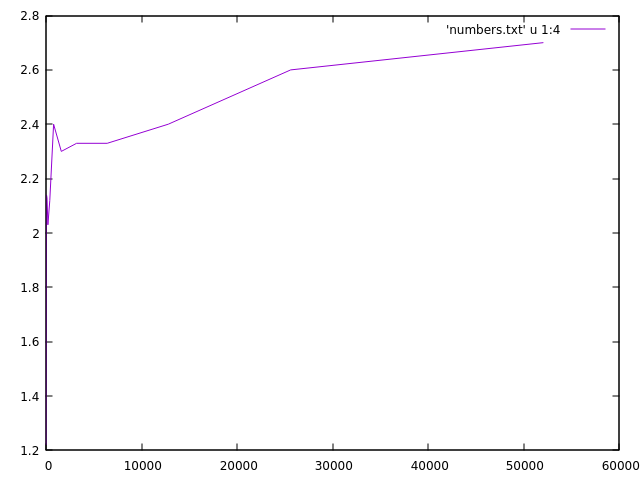
\includegraphics[width=0.8\textwidth]{doubly_simply_ratio.png}
    \caption{The graph describing the evolution of the ratio between doubly and simply linked lists.}
    \label{fig:1}
\end{figure}

As it can be noticed from the graph above, at first, namely for small lists, the unlink and insert operations are executed much faster. However, as the 
array grows, it can be seen as the advantages of the doouble linked list make their presence felt. Since both insert operations are O(1), 
the difference in time execution is given by the unlink operation because the removal of the node can be done instantly without going through the whole list. 

measure the insert only - as expected - very close values - O(1) operation. On average slightly higher for double since there are more lines of code to be executed 

\section*{Difficulties} 

setting the unlink operation for double 
incorrect order for the special cases 

\section*{Conclusion}


\end{document}